\chapter{Experiments and Results}
\label{chapter:experiments}

So far we have discussed the CCD approach in detail. In this chapter,
the experimental evaluation of the CCD algorithm and the naive CCD
tracker will be presented. we apply the CCD approach to three
different kinds of model fitting and object tracking problems:

\begin{enumerate}
\item Contour convergence on still image
\item Track initialization from sift features
\item Track initialization from 3D point cloud
\end{enumerate}

Some experiments have been delivered on the PR2, then we analyze the performance
of the approach in terms of robustness, accuracy and runtime. This is
followed the comparison between the CCD approach and  other
model-based methods.


% by the experimental evaluation of the CCD
% algorithm. presents the evaluation of the naive CCD
% tracker and 

\section{Contour convergence on still image}
\label{sec:ES}

As mentioned in related work, the CCD algorithm is an effective
segmentation method like other model-based segmentation algorithms.

A segmentation means that an image$I: \Omega \subset R^2 \longrightarrow R$
is the partitioning of its domain into homogeneous regions
$\Omega_1,\ldots, \Omega_n \subset \Omega$. In a complex environment,
due to texture, shading, poor contrast and clutter, segmentation is
always a challenging problem in the field of computer
vision(Figure~\ref{fig:flower_m}).

\begin{figure}[htbp]
  \begin{minipage}[t]{0.5\linewidth} 
    \centering 
        \subfloat[the origin image]{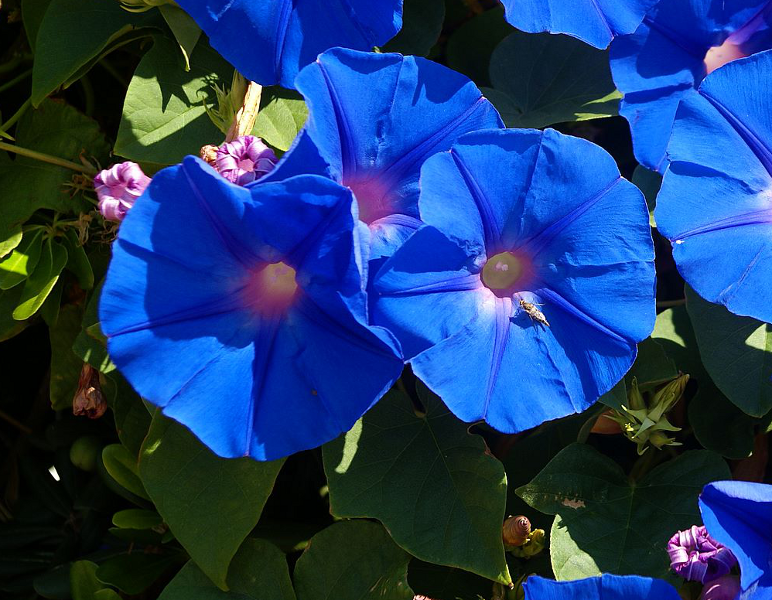
\includegraphics[width=2.5in]{images/segmentation/flowers.png}}
  \end{minipage}% 
  \begin{minipage}[t]{0.5\linewidth} 
    \centering 
    \subfloat[the ROI]{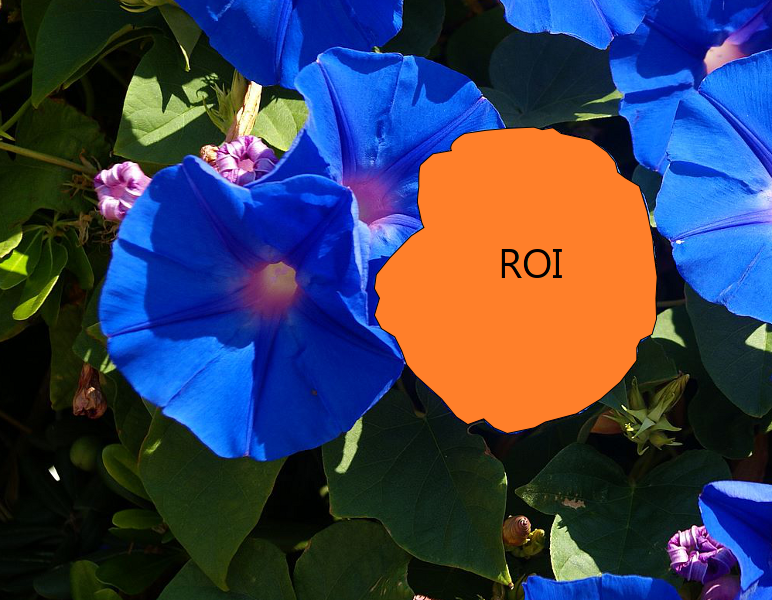
\includegraphics[width=2.5in]{images/segmentation/flowers_m.png}}
  \end{minipage}
\caption[Segmentation a flower petal from a cluster of flowers]{The
  origin image is a little clutter, the border of the ROI in b) can
  not be completely distinguished from the background due poor
  contrast and shading.}
\label{fig:flower_m}
\end{figure}

There are many practical
applications of image segmentation, such as medical imaging, object
tracking, face recognition, fingerprint recognition, machine vison and
so on. In this thesis, we concern its application in object tracking.
In many cases segmentation is the bottleneck when trying to tracking a
object. Many segmentation methods are developed, however, there is not
general solution to the segmentation problem. In the real world,
segmentation problems will often require much domain knowledge before
a successful segmentation can be performed. The CCD algorithm is a
powerful method which is combined with the prior knowledge. By
converting a pure segmentation problem to a problem in pattern
recognition, a large amount of techniques in the field of pattern
recognition are introduced to solve segmentation problems, which are
proved to be effective and helpful. Compared with other segmentation
methods Figure~\ref{fig:seg_compaison}, such as intensive-based method,  cluster method, region-based
method and compression-based methods, the CCD algorithm has following
advantages:
\begin{figure}[htbp] 
  \begin{minipage}[t]{0.5\linewidth} 
    \centering 
    \subfloat[Sobel]{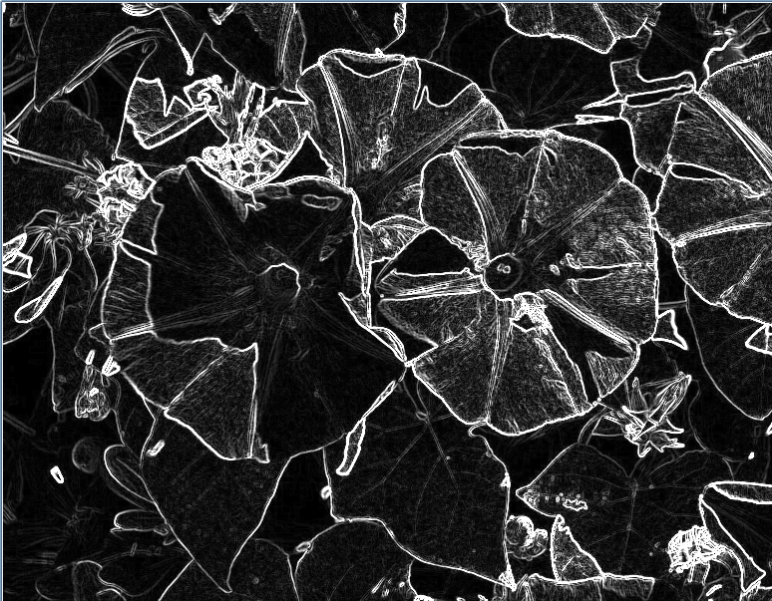
\includegraphics[width=2.5in]{images/flowers_sobel.png}}
  \end{minipage} 
  \begin{minipage}[t]{0.5\linewidth} 
    \centering 
    \subfloat[Watershed algorithm]{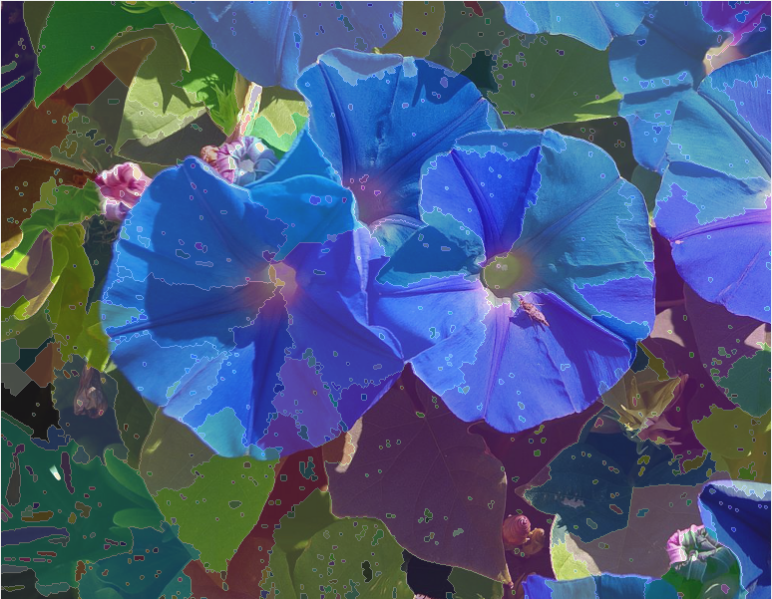
\includegraphics[width=2.5in]{images/flowers_watershed.png}}
  \end{minipage} 
  \begin{minipage}[t]{0.5\linewidth} 
    \centering 
    \subfloat[Graph cut]{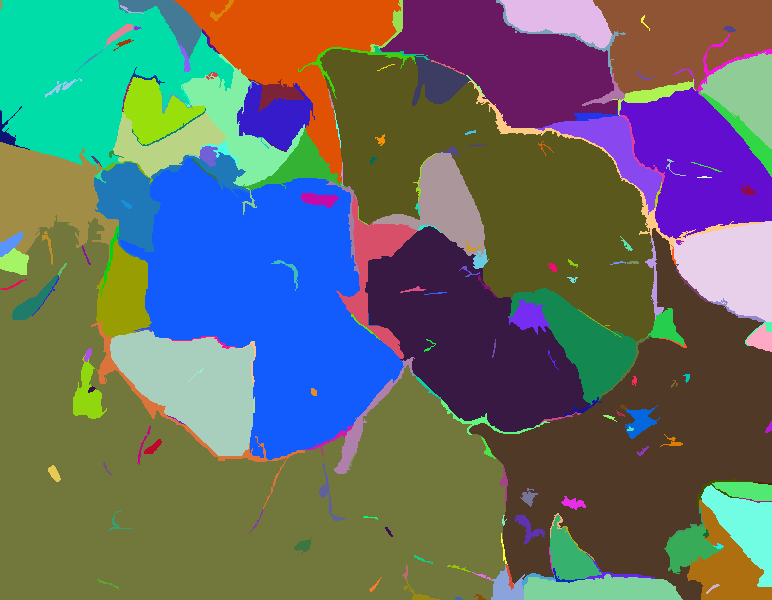
\includegraphics[width=2.5in]{images/flowers_graph.png}}
  \end{minipage} 
  \begin{minipage}[t]{0.5\linewidth} 
    \centering 
    \subfloat[Kmeans++]{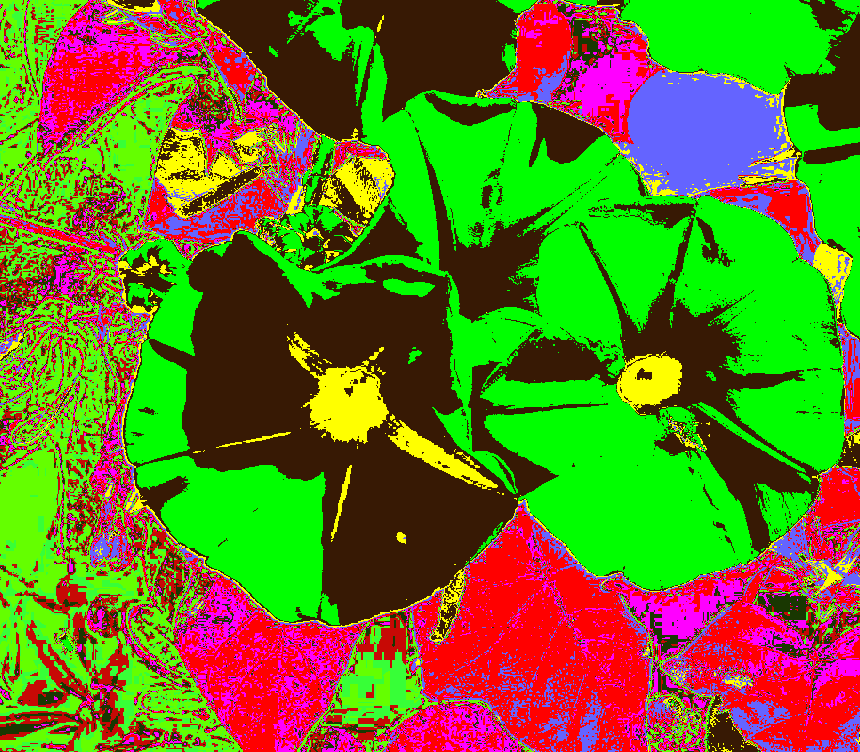
\includegraphics[width=2.5in]{images/flowers_kmeans.png}}
  \end{minipage} 
  \begin{minipage}[t]{0.5\linewidth} 
    \centering 
    \subfloat[Expectation and Maximization]{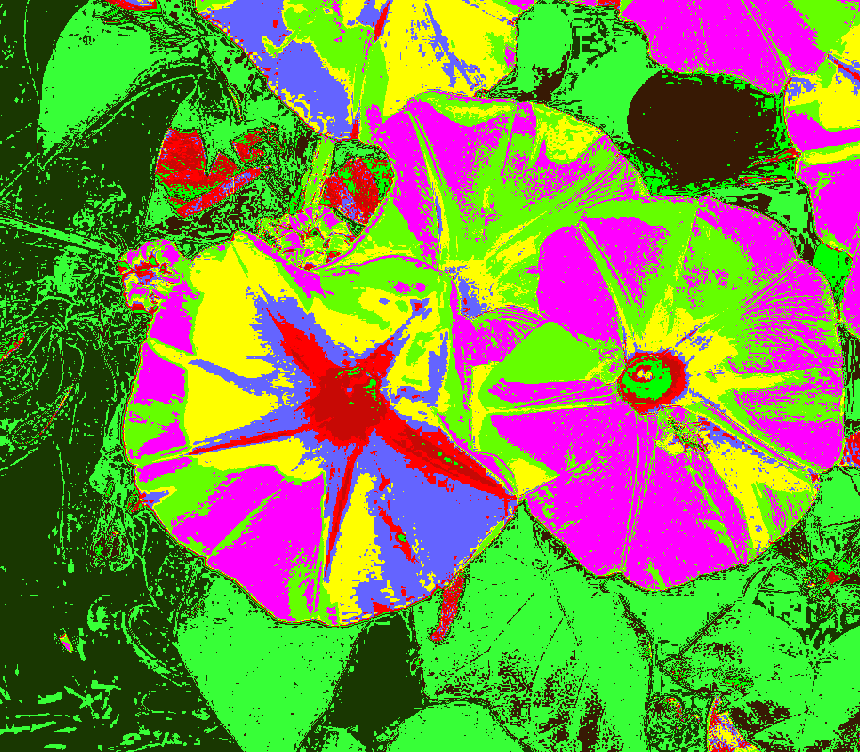
\includegraphics[width=2.5in]{images/flowers_em.png}}
  \end{minipage}
  \begin{minipage}[t]{0.5\linewidth} 
    \centering 
    \subfloat[CCD]{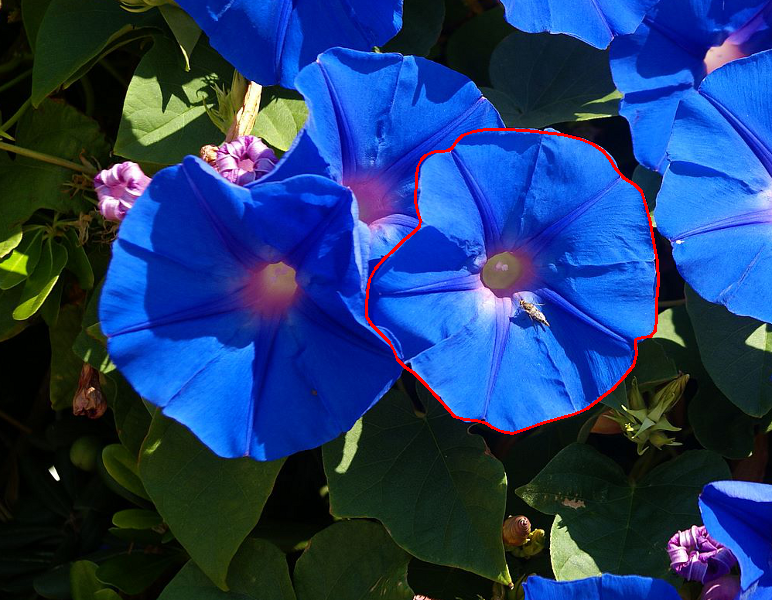
\includegraphics[width=2.5in]{images/flowers_ccd.png}}
  \end{minipage}% 
\caption[Resulting images after applying some segmentation methods]{a)
  Edges are detected by a gradient-based algorithm~\cite{scharr2000optimal}. b) Watershed algorithm takes an image as a
  topographic relief. c) Segment an image by defining a predicate for
  measuring the evidence for a boundary between two regions using a
  graph-based representation of the
  image~\cite{felzenszwalb2004efficient}. d) K-means++ algorithm is a
  cluster-based segmentation algorithm~\cite{arthur2007k}. e)
  Segmentation result of Expectation-Maximization (EM) algorithm,
  usually it is initialized by K-means algorithm~\cite{bishop2006pattern}. f) the contour segmented by the CCD
  algorithm introduced in this thesis.}
\label{fig:seg_comparison}
\end{figure}

\begin{itemize}
\item restrict segmentation problem to a limited explicit region, it is helpful
  to decrease the computation cost.
\item probabilistic representation of the variation of the registered
  samples could be easily given, thus statistical inference between
  the model and the image will be applied. All these are helpful to
  improve the segmentation results.
\item The CCD algorithm achieves sub-pixel accuracy and high
  robustness because only a relatively small fraction of the pixels is
  taken into account in the end of iteration.
\end{itemize}

In the following, we apply the proposed CCD algorithm to 4 kind of
objects:
\begin{enumerate}
\item Segmentation of a spherical object
\item Segmentation of a 3-D object
\item Segmentation of a transparent object
\item Fitting a rigid wire frame.
\end{enumerate}

\subsection{Segmenation of a ball}
\label{sec:sb}
Like other contour-based method, we model a contour of the ball as the
prior knowledge. Because the contour for a rigid spherical object is a
circle, besides manually initialization, we can use some built-in function in
OpenCV library to generate the contour with given center and
radius. According to the definition of prior distribution, it is required
that the hypothesis is in the range of the variation of
registered sample, namely, the initial contour can not be too far away
from the observed object.

\begin{figure}[htbp] 
  \begin{minipage}[t]{0.5\linewidth} 
    \centering 
        \subfloat[iteration 1]{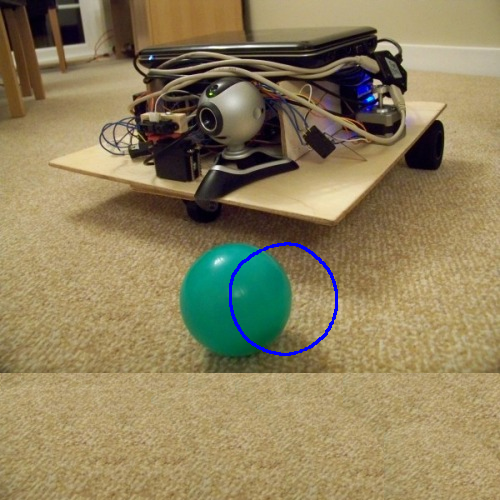
\includegraphics[width=2.5in]{images/ball/0.png}}
  \end{minipage}% 
  \begin{minipage}[t]{0.5\linewidth} 
    \centering 
    \subfloat[iteration 3]{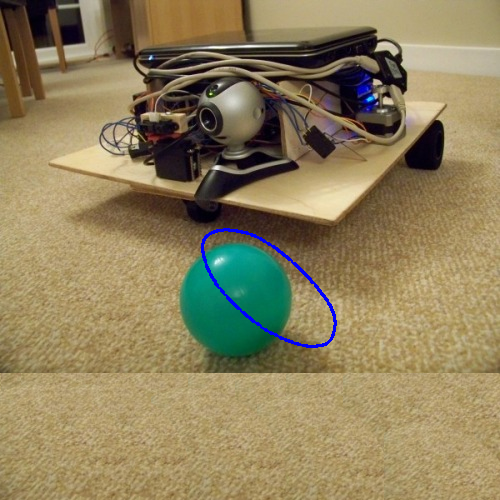
\includegraphics[width=2.5in]{images/ball/2.png}}
  \end{minipage} 
  \begin{minipage}[t]{0.5\linewidth} 
    \centering 
    \subfloat[iteration 7]{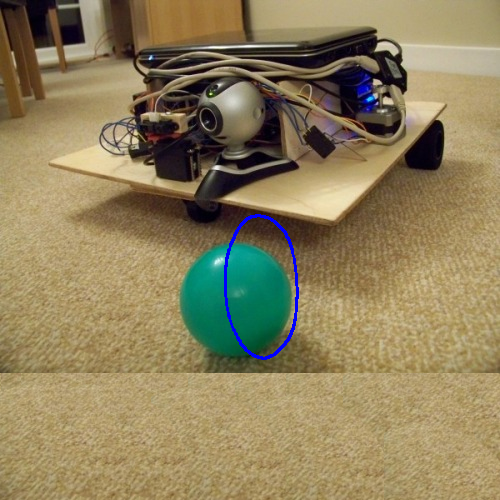
\includegraphics[width=2.5in]{images/ball/6.png}}
  \end{minipage} 
  \begin{minipage}[t]{0.5\linewidth} 
    \centering 
    \subfloat[iteration 16]{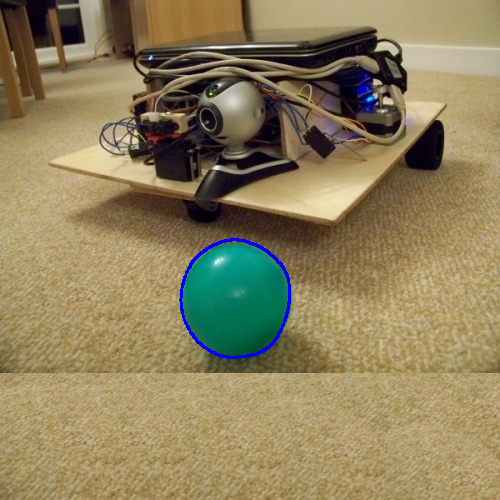
\includegraphics[width=2.5in]{images/ball/15.png}}
  \end{minipage} 
\caption[Segmentation of a ball]{There is a translation between the
  initial hypothesis and the contour of the observed object. However, It is
  mandatory that the initial contour encompass at least part surface
  of the object being learning. In the beginning, the uncertainty of
  the contour is very large, so the contour is always changing in
  affine-space, after several iteration, it starts to converge and
  successfully detects the contour.
\label{fig:sab}
}
\end{figure}

In Figure~\ref{fig:sab}, we intentionally set a hypothesis which is far away
from the ball, but after about 15 iteration, we successfully fit the
contour the edge of the ball. For the sake of a ground truth we need
investigate the pixels used in the iterations. The Figure~\ref{fig:pon} shows
that only a small number of pixels is taken into account after the
contour starts to converge. However, these pixels contain the
necessary information for refining the fitting. Because the pixels used
to compute become less and less, at last, it is supposed that
only a small number of pixels near the boundary are considered, thus the
CCD algorithm can achieve high sub-pixel accuracy.

\begin{figure}[htbp] 
  \begin{minipage}[t]{0.5\linewidth} 
    \centering 
    \subfloat[iteration 1]{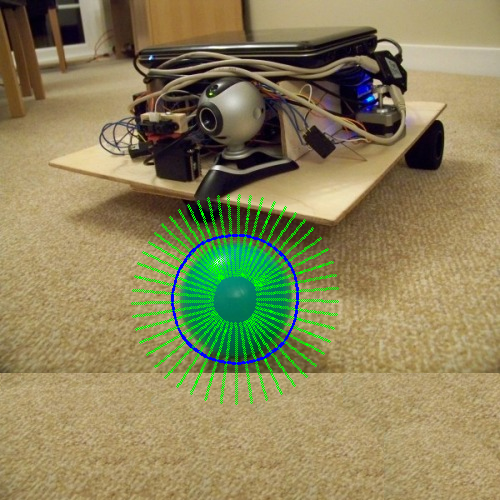
\includegraphics[width=2.5in]{images/ball_normal/0.png}}
  \end{minipage}% 
  \begin{minipage}[t]{0.5\linewidth} 
    \centering 
    \subfloat[iteration 3]{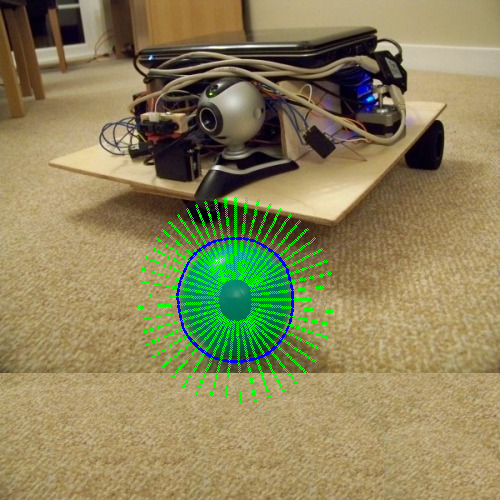
\includegraphics[width=2.5in]{images/ball_normal/1.png}}
  \end{minipage} 
  \begin{minipage}[t]{0.5\linewidth} 
    \centering 
    \subfloat[iteration 5]{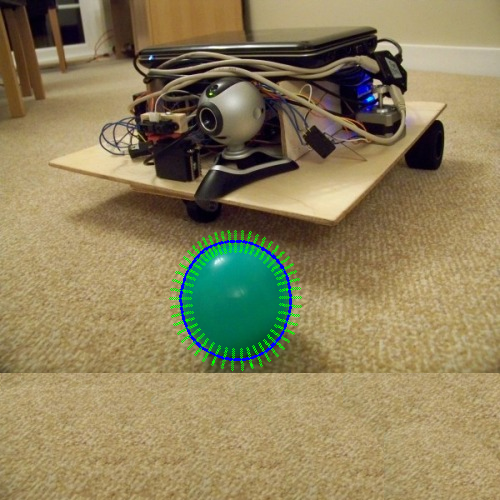
\includegraphics[width=2.5in]{images/ball_normal/3.png}}
  \end{minipage} 
  \begin{minipage}[t]{0.5\linewidth} 
    \centering 
    \subfloat[iteration 6]{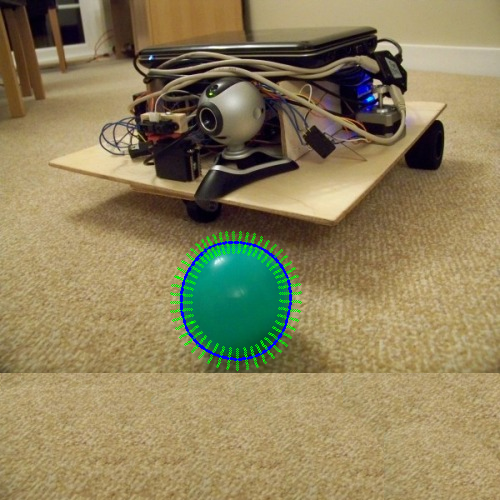
\includegraphics[width=2.5in]{images/ball_normal/4.png}}
  \end{minipage} 
\caption[Pixels used in each iteration]{Generally, compared with other
  algorithm, the pixels used in the CCD algorithm are much less. In
  the end of convergence, only a few pixels are taken into
  account. This leads to performance and accuracy improvement.}
\label{fig:pon}
\end{figure}


\subsection{Segmentation of a 3-D obejct}
\label{sec:s3o}
In the experiments of segmentation of a spherical object, a planar
affine space of contour is generated. It works very well because the
contour of the ball is always a circle, there is not parallax effect
for such objects. In this case, a 6-dimension model parameters vector
can cope with basic geometrical transformation of a object. However,
clearly a 6-dimension model parameters vector can not be expected to
suffice for non-planar surfaces. Imagine such a scenario, we generate the  planar affine
space contour of a non-planar cube in the fist view. In the
subsequent view the outline of the cube does not lie in the old
space. Due the parallax effect the a mismatch in the fitted contour
will be detected. This can be evidenced in the fitting experiment (Figure~\ref{fig:box_mismatch}).
\begin{figure}[htbp]
  \begin{minipage}[t]{0.5\linewidth} 
    \centering 
    \subfloat[]{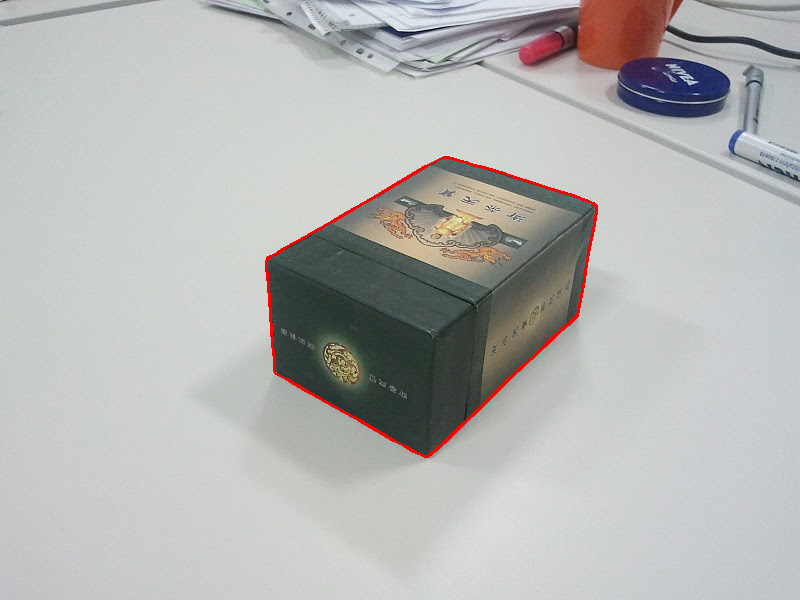
\includegraphics[width=2.5in]{images/box1.png}}
  \end{minipage}% 
  \begin{minipage}[t]{0.5\linewidth} 
    \centering 
    \subfloat[]{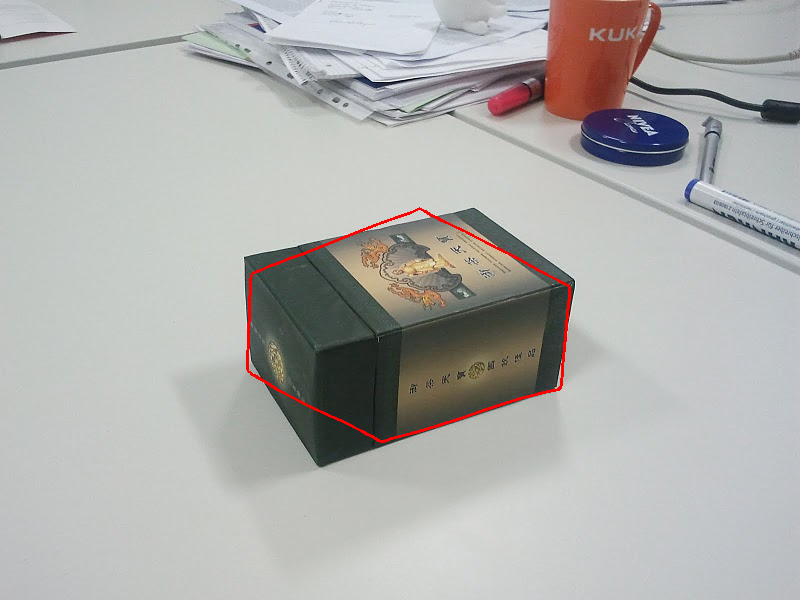
\includegraphics[width=2.5in]{images/box2_mismatch.png}}
  \end{minipage} 
  \caption[Planar space can not encompass a general non-planar
  contour]{a) A planar affine space of contours has been fitted from
    the outline of the first view of the cuboid. b) As the viewpoint
    is changed, the outline of the cuboid in the subsequent view does
    not lie in the affine space, which causes visible mismatch in the
    fitted contours.}
\label{fig:box_mismatch}
\end{figure}


The new 3-dimensional affine shape-space with 8 degree of freedom,
made up of the 6-parameter planar affine space and a two-parameter
extension, is designed to cope with such problem. Two added components
account for the depth variation that is not visible in the template
view. If tacking the two new parameters to the shape matrix, the form
of shape matrix for 3-dimensional case can be given by
\begin{equation}
  \label{eq:4.18}
  A =
  \begin{bmatrix}
    1 & 0 & P_0^x & 0 & 0 & P_0^y & P_0^z & 0\\
    0 & 1 & 0 & P_0^y & P_0^x & 0 & 0  & P_0^z
  \end{bmatrix}
\end{equation}

\begin{figure}[htbp]
  \begin{minipage}[t]{0.5\linewidth} 
    \centering 
    \subfloat[]{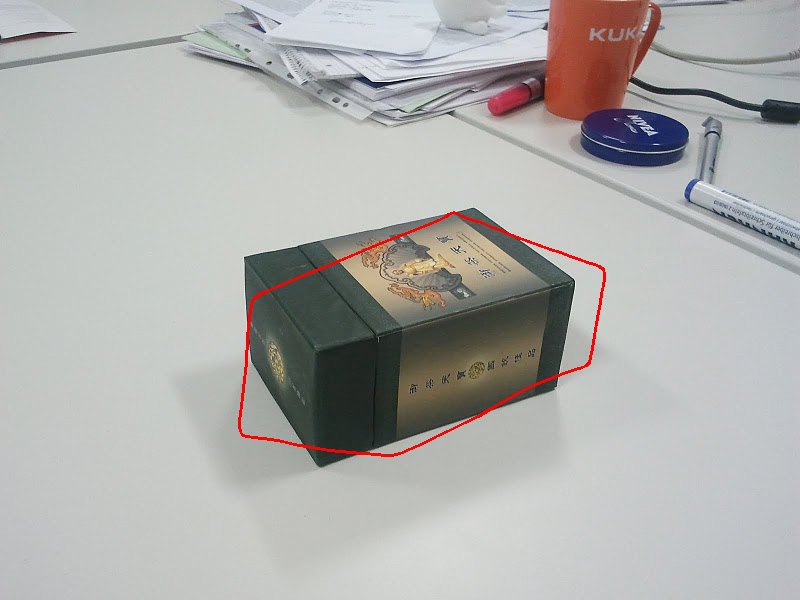
\includegraphics[width=2.5in]{images/box2_3d.png}}
  \end{minipage}% 
  \begin{minipage}[t]{0.5\linewidth} 
    \centering 
    \subfloat[]{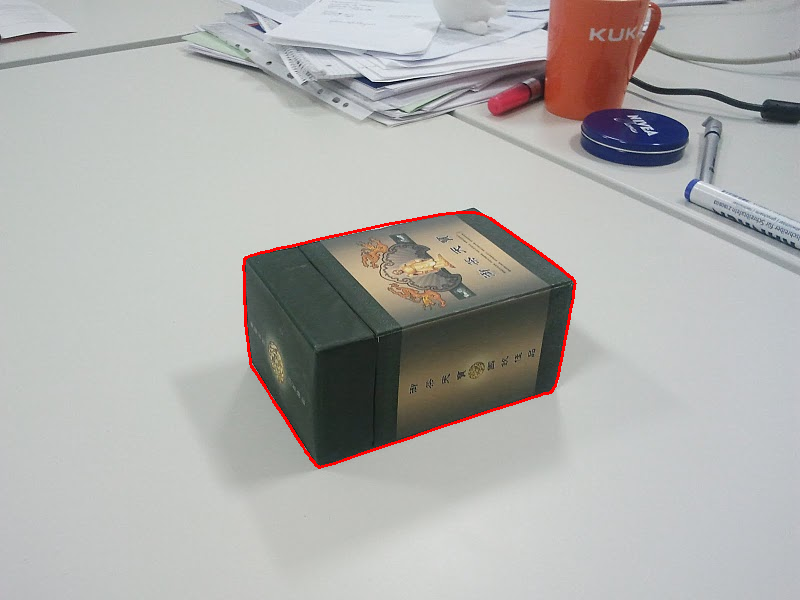
\includegraphics[width=2.5in]{images/box2_ok.png}}
  \end{minipage} 
  \caption[Non-planar contour has been successfully fitted]{The
    contour of a cube which could not be encompassed in a planar
    affine shape-space now falls within a suitably constructed 3D affine space.}
\label{fig:box_match}
\end{figure}

The three-dimensional affine shape-space model parameters have
the following interpretation

\begin{equation}
  \label{eq:4.19}
  \mathbf{\Phi} =  (T_1, T_2, M_{11} - 1, M_{22} - 1, M_{21}, M_{12}, \nu_1, \nu_2)
\end{equation}

The expanded space now encompasses the outlines of all views of the three-dimensional
outline, evidenced by Figure~\ref{fig:box_match}. At last, we do
another experiments for a object with an irregular shape~\ref{fig:container}. This
demonstrates that the CCD works well for 3-D non-planar object.

\begin{figure}[htbp] 
  \begin{minipage}[t]{0.5\linewidth} 
    \centering 
    \subfloat[iteration 1]{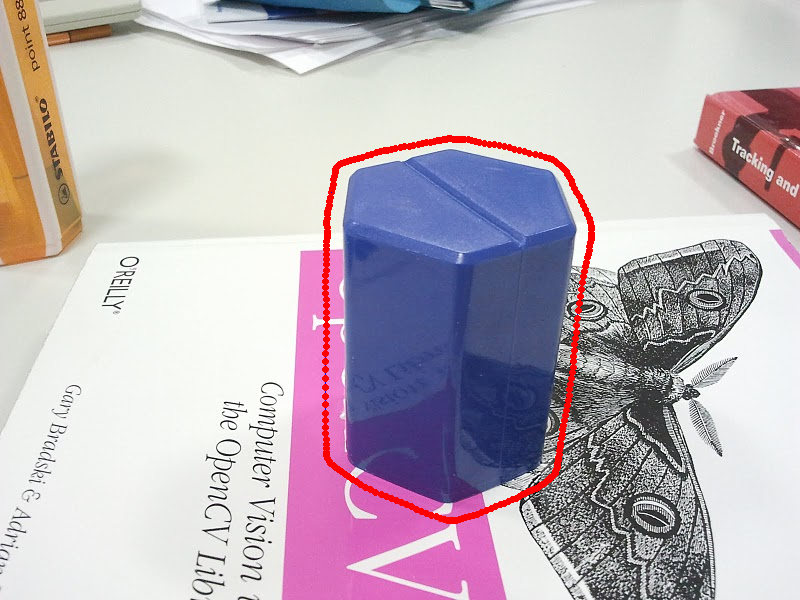
\includegraphics[width=2.5in]{images/container/0.png}}
  \end{minipage}% 
  \begin{minipage}[t]{0.5\linewidth} 
    \centering 
    \subfloat[iteration 2]{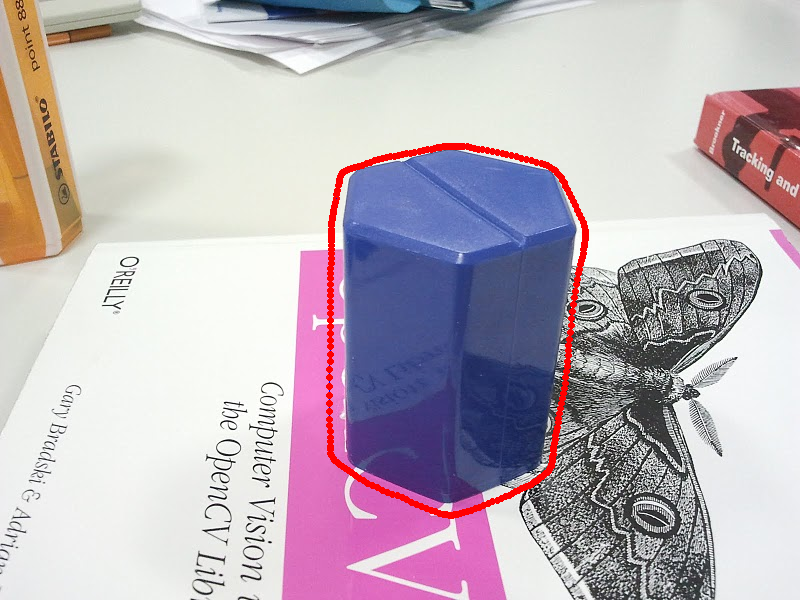
\includegraphics[width=2.5in]{images/container/1.png}}
  \end{minipage} 
  \begin{minipage}[t]{0.5\linewidth} 
    \centering 
    \subfloat[iteration 4]{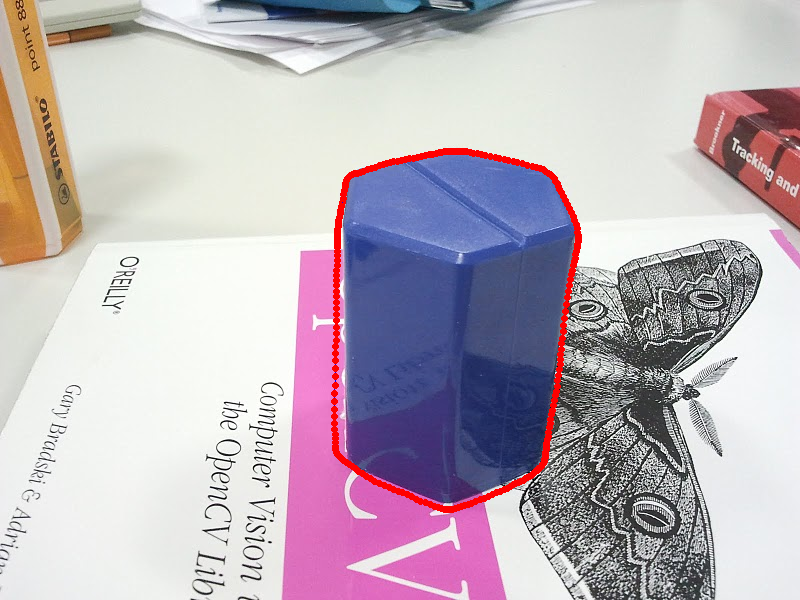
\includegraphics[width=2.5in]{images/container/2.png}}
  \end{minipage} 
  \begin{minipage}[t]{0.5\linewidth} 
    \centering 
    \subfloat[iteration 7]{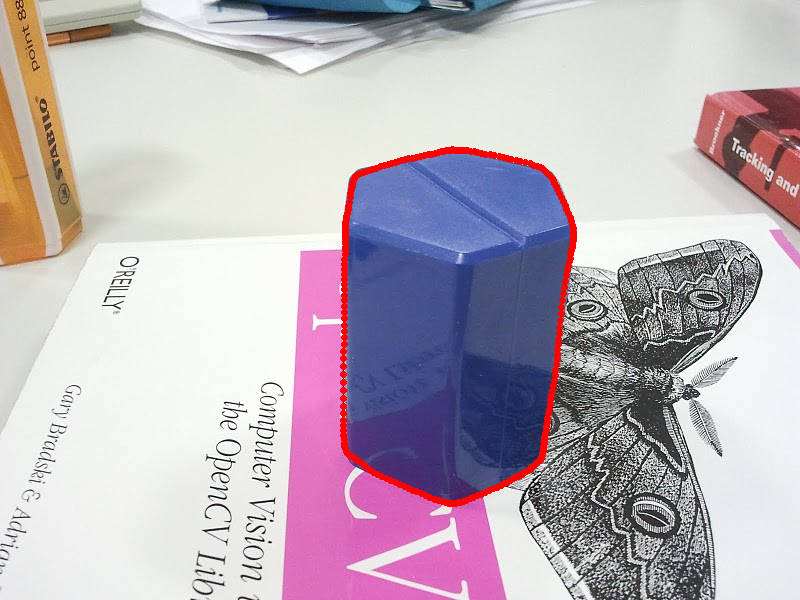
\includegraphics[width=2.5in]{images/container/5.png}}
  \end{minipage} 
\caption[Three-dimensional affine shape-space for rigid object]{The
  non-planar polyhedron is encompassed by a 3D affine space}
\label{fig:container}
\end{figure}

\subsection{Segmentation of transparent objects}
\label{sec:sto}
In this thesis, local statistical information is collected in terms of
pixel intensity in the vicinity of a contour, this leads to a poor
result for transparent objects. In this experiment, the
target is a cola bottle whose upper part is nearly transparent and the
lower part is opaque. The result in Figure~\ref{fig:cola} shows that the CCD algorithm
can segment the lower part but can not completely encompass the contour in the
upper part. However, because the model only have 6 (or 8
for 3-dimensional object) degree of freedom, the convergence of other
part will effect the fitting in the transparent part such that we can
detect that the convergence happens in the transparent part.


\begin{figure}[htbp] 
  \begin{minipage}[t]{0.5\linewidth} 
    \centering 
    \subfloat[iteration 1]{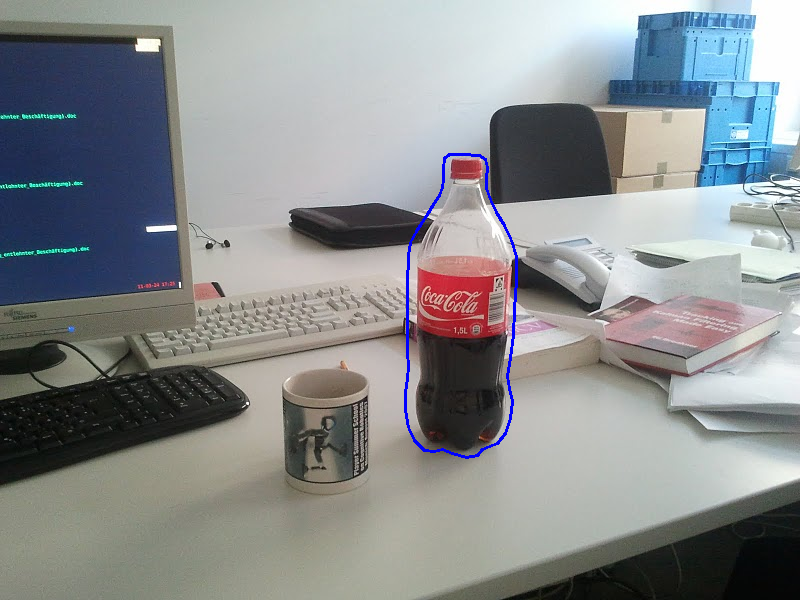
\includegraphics[width=2.5in]{images/bottle/0.png}}
  \end{minipage}% 
  \begin{minipage}[t]{0.5\linewidth} 
    \centering 
    \subfloat[iteration 2]{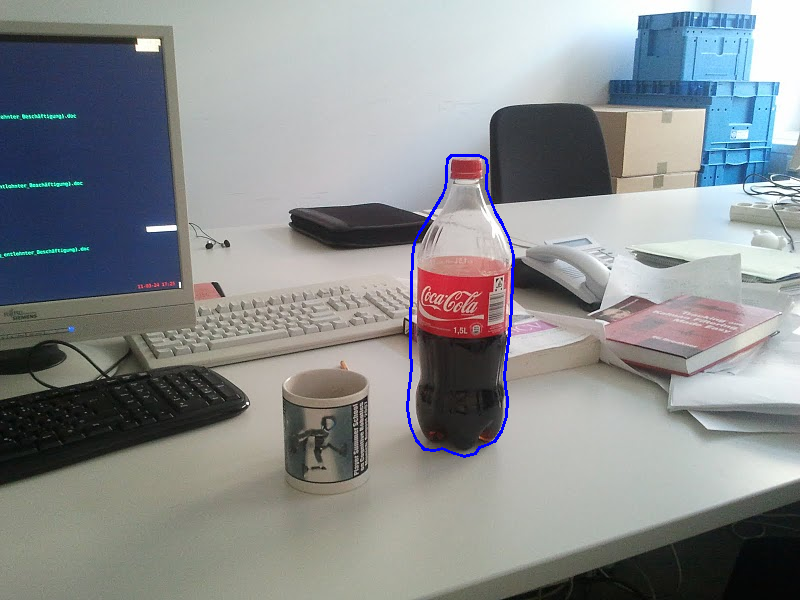
\includegraphics[width=2.5in]{images/bottle/1.png}}
  \end{minipage} 
  \begin{minipage}[t]{0.5\linewidth} 
    \centering 
    \subfloat[iteration 3]{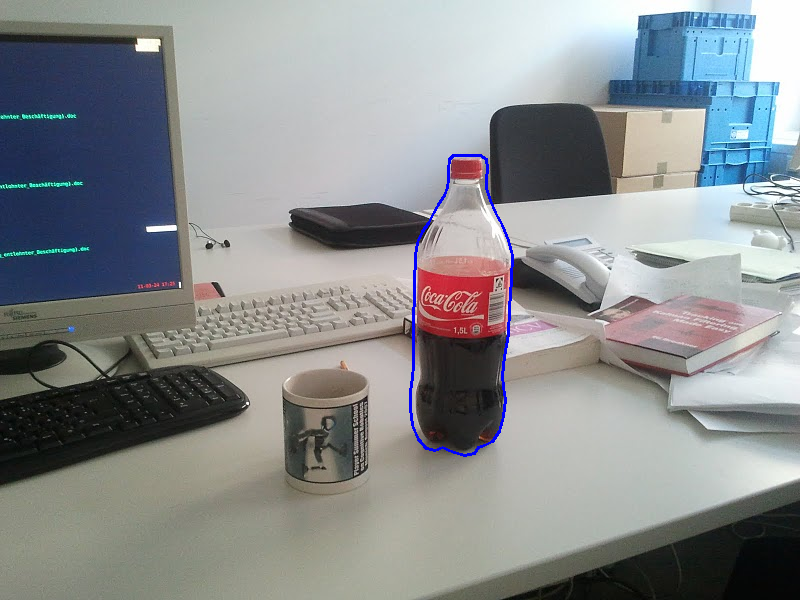
\includegraphics[width=2.5in]{images/bottle/2.png}}
  \end{minipage} 
  \begin{minipage}[t]{0.5\linewidth} 
    \centering 
    \subfloat[iteration 21]{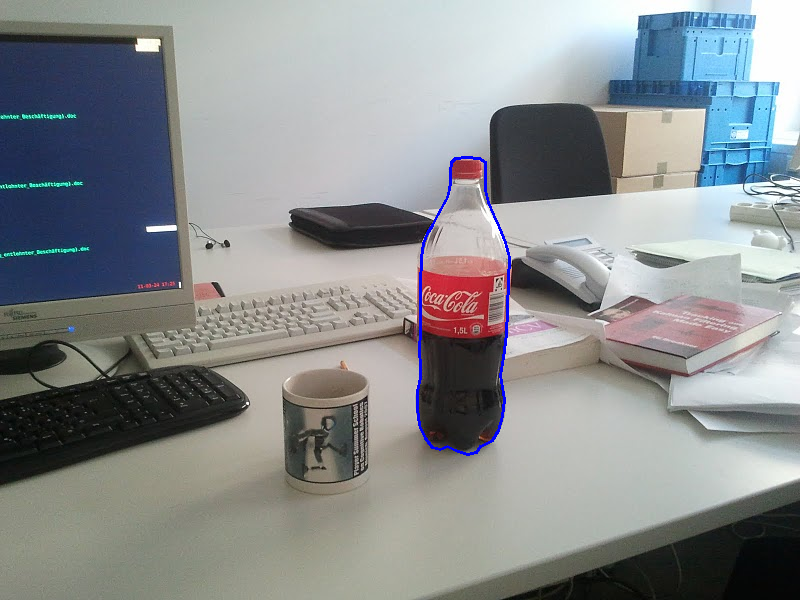
\includegraphics[width=2.5in]{images/bottle/20.png}}
  \end{minipage} 
\caption[Segmentation of a transparent bottle]{in image (d), Due the shadow and poor
contrast, the contour does not completely attach to the edge of the
bottom. Moreover, in the transparent part of the bottle, the outline
closely attaches to the edge in the left but stays away from the edge
in the right. The transparency leads to the difficulties. }
\label{fig:cola}
\end{figure}


\subsection{Fitting a rigid wire frame}
\label{sec:fdo}
In the following, we fit a rigid wire frame model to the image
depicted in Figure~\ref{fig:wireframe}.  The degrees of freedom
are the 8 pose parameters. This experiment demonstrates that the CCD
algorithm is not only able to exploit object contours, but it can also
use internal model edges separating multiple, possibly dependent,
image regions.  The CCD algorithm reliably estimates the pose of the box despite
the partial occlusion.

\begin{figure}[htbp] 
  \begin{minipage}[t]{0.5\linewidth} 
    \centering  
    \subfloat[iteration 1]{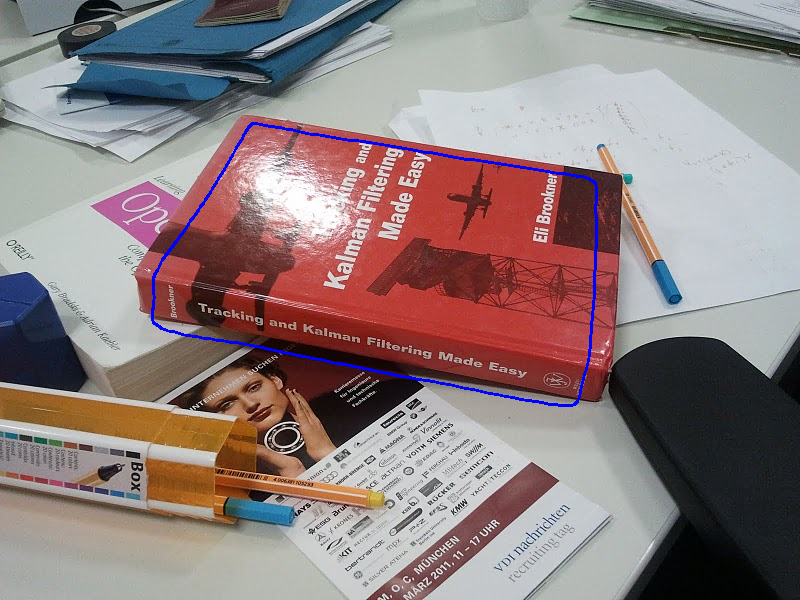
\includegraphics[width=2.5in]{images/book/0.png}}    
  \end{minipage}% 
  \begin{minipage}[t]{0.5\linewidth} 
    \centering 
    \subfloat[iteration 2]{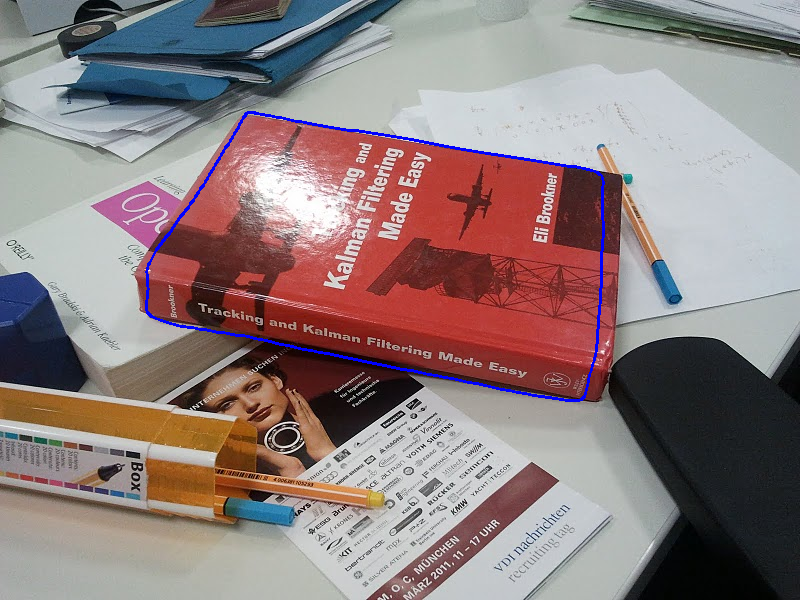
\includegraphics[width=2.5in]{images/book/1.png}}
  \end{minipage} 
  \begin{minipage}[t]{0.5\linewidth} 
    \centering 
    \subfloat[iteration 3]{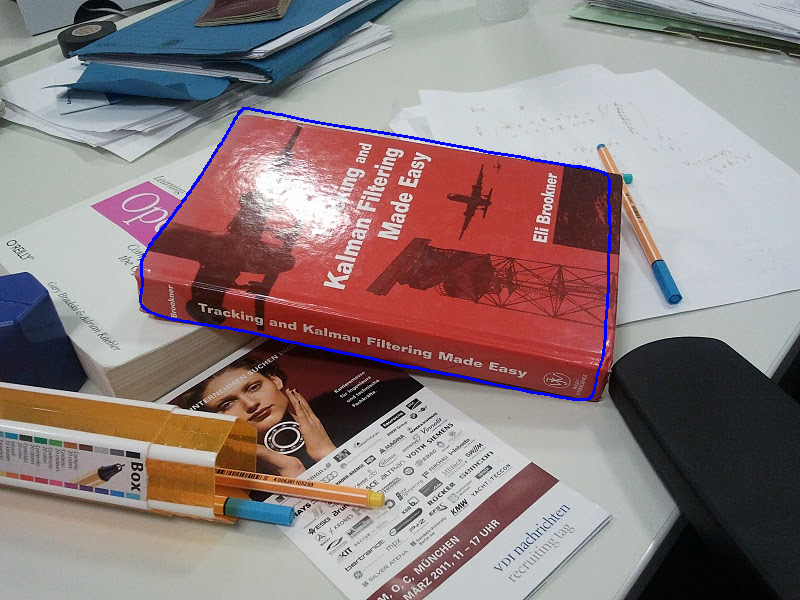
\includegraphics[width=2.5in]{images/book/2.png}}
    \label{subfig:iteration 3}
  \end{minipage} 
  \begin{minipage}[t]{0.5\linewidth} 
    \centering 
    \subfloat[iteration 14]{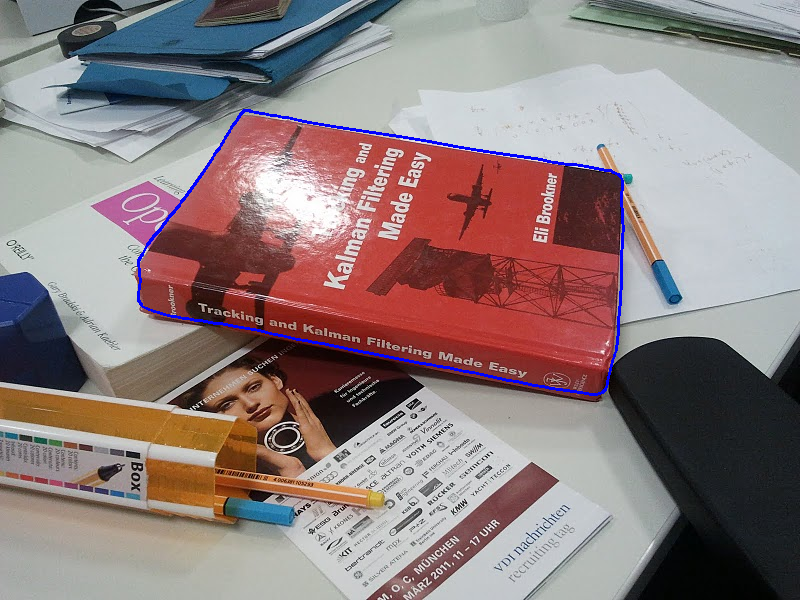
\includegraphics[width=2.5in]{images/book/13.png}}
  \end{minipage}
  \begin{minipage}[t]{\linewidth} 
    \centering 
    \subfloat[segmentation of edge-based algorithm]{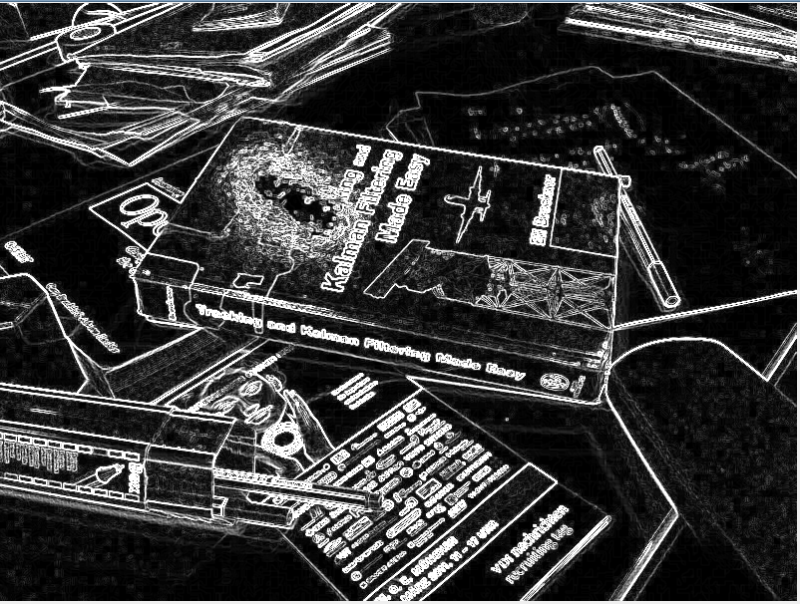
\includegraphics[width=0.8\linewidth]{images/book/book_sobel.png}}
  \end{minipage} 
\caption[Fitting a rigid wire frame in a inhomogeneous background]{The book
  is located in a partially occluded background. From (a)-(d), despite
the variation of the illumination and contrast, the CCD algorithm
accurately fits a wire frame model to the image data. In (e), here the
edge-based algorithm yields some errors.}
\label{fig:wireframe}
\end{figure}


\section{Track initialization from SIFT features}
\label{sift_init}
Scale-invariant feature transform (or SIFT) is an algorithm to detect
and describe local features in images.  It is widely used to solve
many problems in the field of Computer Vision, such as object
recognition, robotic mapping and navigation, video tracking, and match
enmoving. There are four key stages in the sift algorithm~\cite{lowe2004distinctive}:
\begin{enumerate}
\item \textbf{Scale-invariant feature detection}: an image is transformed into
  a collection of vectors which are scale-invariant. By applying a difference-of-Gaussian
function to a series of smoothed and resampled images, potential
interest can be identified.
\item \textbf{Keypoint localization and indexing}: keypoints are selected at given
  candidate location, then store SIFT keys and identifying matching keys from the new image
\item \textbf{Orientation assignment}:  based on local image gradient
  directions each keypoint is assigned one or more orientations.
\item \textbf{Keypoint descriptor}: measure the local image gradients
  at the selected scale in the region around each keypoint
\end{enumerate}


The SIFT keypoints and features are local and based on the appearance
of the object at particular interest points. The SIFT algorithm has following
features and advantages:
\begin{itemize}
\item invariant to image scale and rotation, robust to changes in
  illumination and minor changes in viewpoint
\item highly distinctive, easy to extract,allow for correct object
  identification and easy to match against a database of local
  features. 
\item need few features (as few as 3) from an object to compute its location
  and pose. Computation cost is moderate on modern computer hardware.
\end{itemize}

Based on these features, SIFT is usable for object recognition, the
steps are given below.
\begin{itemize}
\item Extract SIFT features from a series of input template image,
  then store these features into a database.
\item Given a new input image, after training, the features in
  the image are matched to the SIFT feature database obtained from the
  training images.
\end{itemize}

In this thesis, we plan to use the SIFT algorithm to initialize the
contour of an object. Assume we have marked the boundary points in the
training images. In order project these boundary points to a image
being studied, it is essential to estimate the homography between the
images. The SIFT is helpful for realize this. However, SIFT matching
in the step 2 above might leads to lots of "false" matches. In order
to evaluate the homography, firstly we have to exclude the
mismatches. 

RANSAC is a good approach for this and ideal partner of SIFT. It is a
iterative process by randomly select enough matches to fit
homography. It contains following stages~\cite{fischler1981random}.
\begin{itemize}
\item  Randomly select a sample of matched points and instantiate the
  model from this subset
\item Determine the set of data points that are within a distance
  threshold of the homography. The set is the consensus set of the sample
  and defines the inliers.
\item If the size of the set (e.g. the number of inliers) is greater
  than some threshold, re-estimate the homography using all the matched
  points and terminate. Otherwise, select a new subset and repeat the
  above.
\item After some trials the largest consensus set is selected, and the
  homography is re-estimated using all the points in the subset.
\end{itemize}
One fast way to compute the homography in a least squares sense is to use the Normalized
Direct Linear Transform (normalized
DLT)~\cite{hartley2003multiple}. The Normalized DLT algorithm computes
a homography for a projective transformation by using at least 4 point
correspondences and then minimizing corresponding norm.

After obtaining the homography between the template image and the
image being studied, the contour of object can be easily projected
into the target image to obtain the estimate of the contour
position. This is illustrated in Figure~\ref{fig:sift} on page
\pageref{fig:sift} and Figure~\ref{fig:sift_result} on page
\pageref{fig:sift_result}. Note that because SIFT is only invariant for
minor changes in view points, the method does not always work for
non-planar object which has different viewpoint from the one in the
template image.

\begin{figure}[htbp]
  \centering
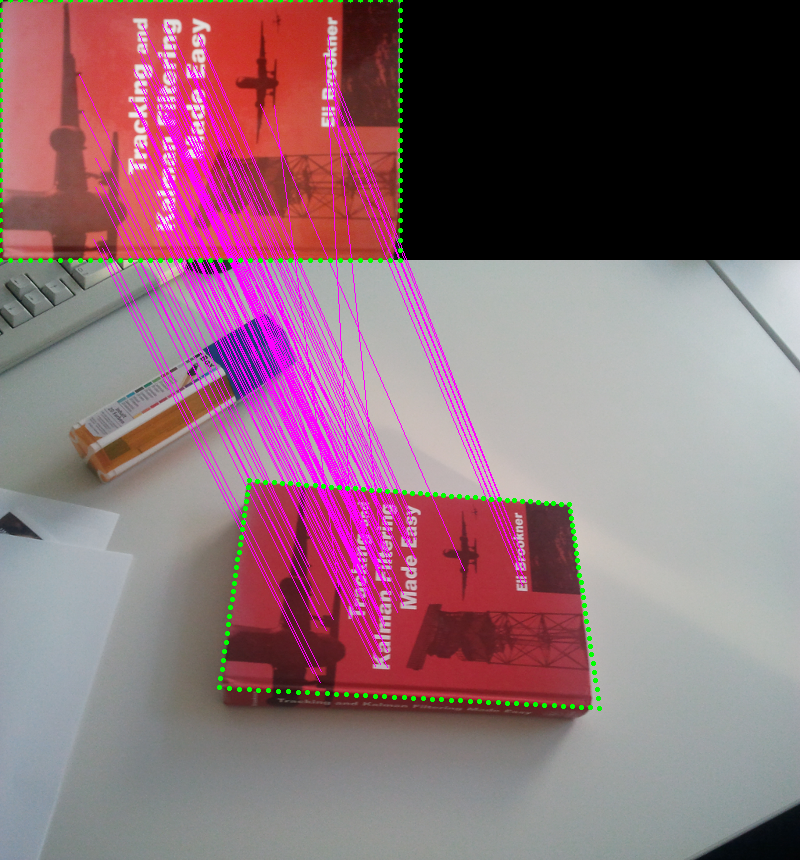
\includegraphics[width=\linewidth]{images/sift.png}
\caption[Contour initialization using the SIFT algorithm]{The image in
  the upper-left corner is a template. It is projected into the bottom
  image. The green points in the template encompass the
  contour of the observed object.The red lines are used to connect the matching feature
  points. Obviously, the outliers are excluded using some algorithms
  (e.g. RANSAC). Then the homography can be estimated from these matching
  feature points.  After applying a perspective
  transformation to the template, the source contour is projected to
  the wrapped one in the bottom, which is used as the control points
  in the CCD algorithm.
  }
\label{fig:sift}
\end{figure}

\begin{figure}[htbp]
  \centering
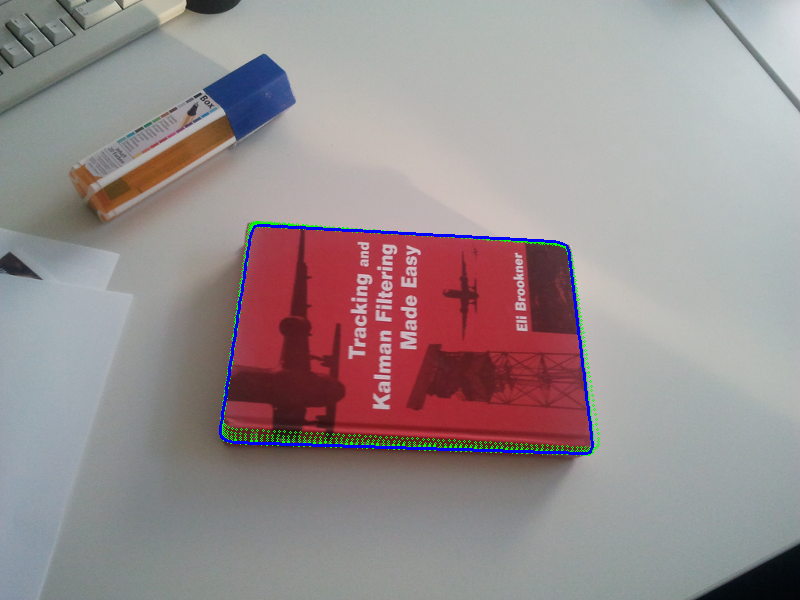
\includegraphics[width=\linewidth]{images/sift_result.png}
\caption[The contour obtained using the CCD algorithm converges to the
edge of the book]{After 8 iterations, the contour obtained in Figure
  ~\ref{fig:sift} converges to the edge of the book. However, in our
  implementation, the SIFT algorithm can only cope with 2-Dimensional
  local features, but actually the book on the desk is a non-planar
  object. Therefore, the result is not as good as expected.}
\label{fig:sift_result}
\end{figure}

The model hypothesis is obtained by applying the CCD algorithm to a
frame of a video sequence. In the following experiments, we can test
our naive CCD tracker on PR2, the result is demonstrated in Figure
~\ref{fig:siftracker} 

\begin{figure}[htbp]
  \begin{minipage}[t]{0.5\linewidth} 
    \centering  
    \subfloat[Sampled frame 1]{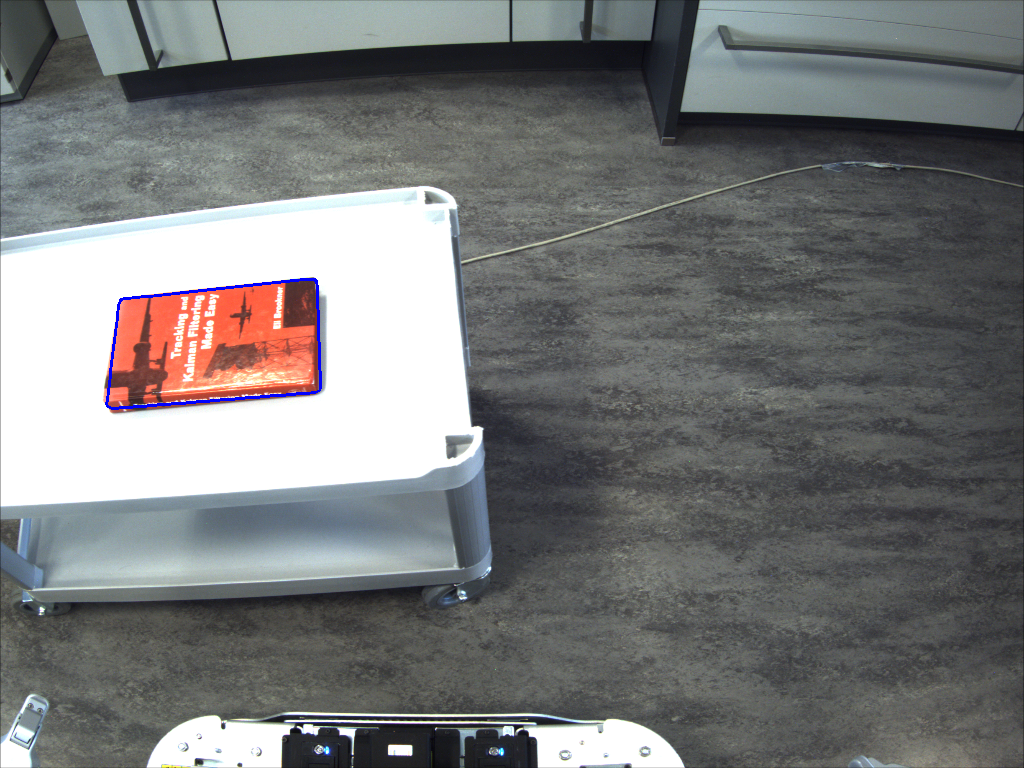
\includegraphics[width=2.5in]{images/sift/1.png}}    
  \end{minipage}% 
  \begin{minipage}[t]{0.5\linewidth} 
    \centering 
    \subfloat[Sampled frame 2]{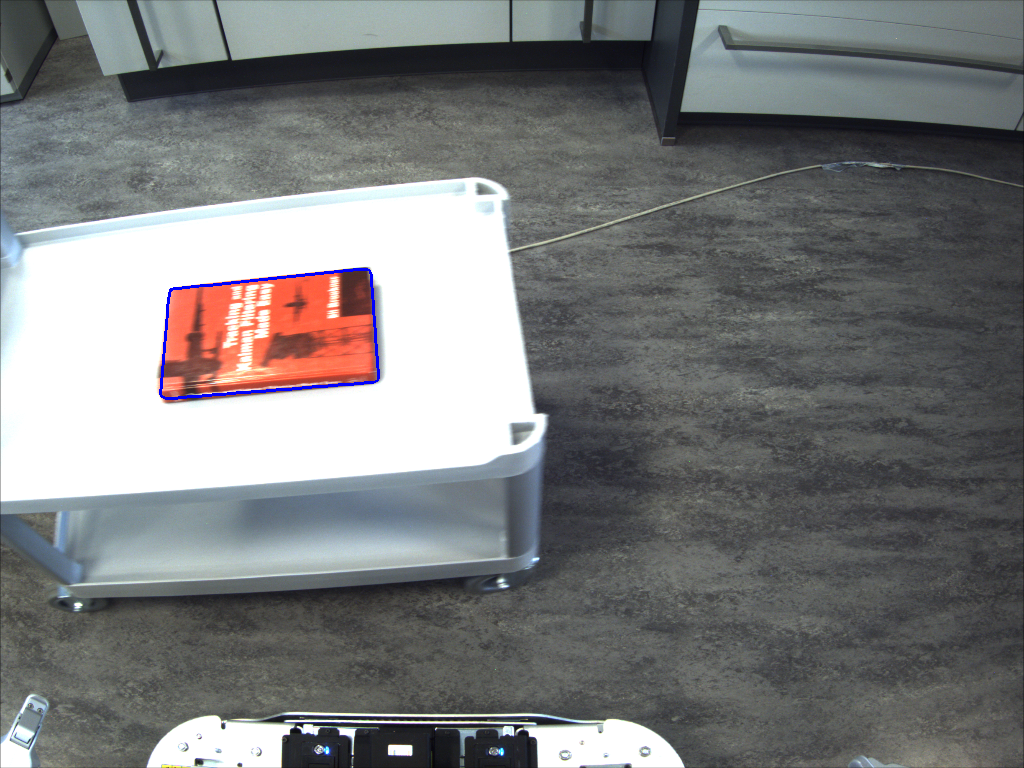
\includegraphics[width=2.5in]{images/sift/10.png}}
  \end{minipage} 
  \begin{minipage}[t]{0.5\linewidth} 
    \centering 
    \subfloat[Sampled frame 3]{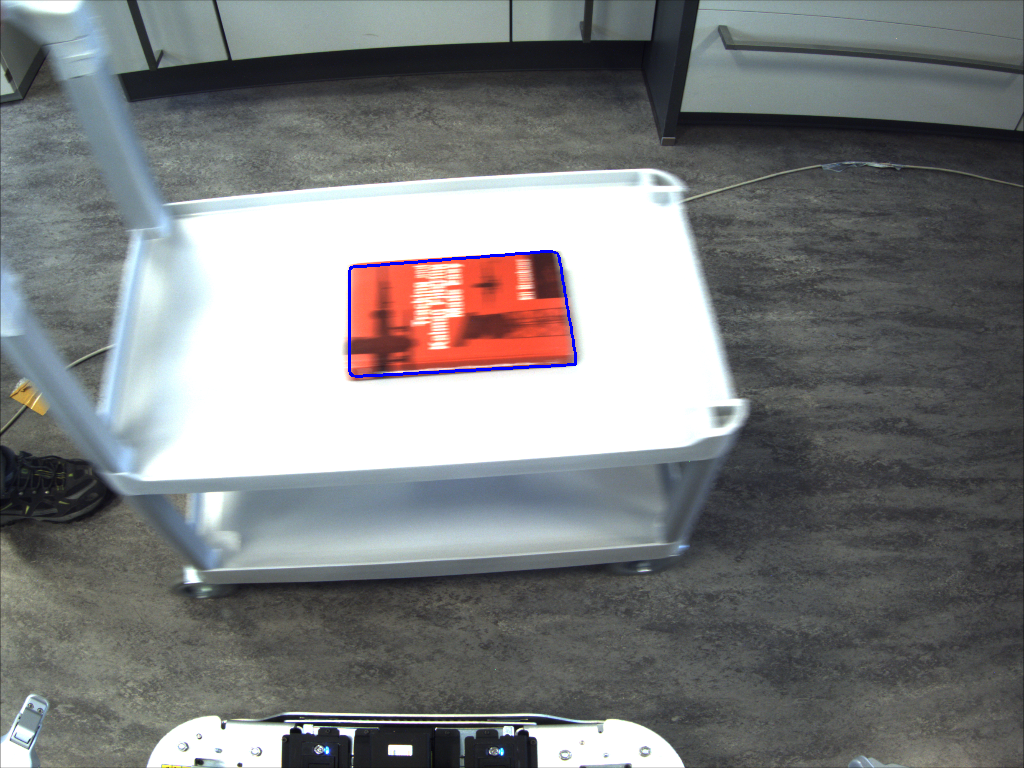
\includegraphics[width=2.5in]{images/sift/30.png}}
    \label{subfig:iteration 3}
  \end{minipage} 
  \begin{minipage}[t]{0.5\linewidth} 
    \centering 
    \subfloat[Sampled frame 4]{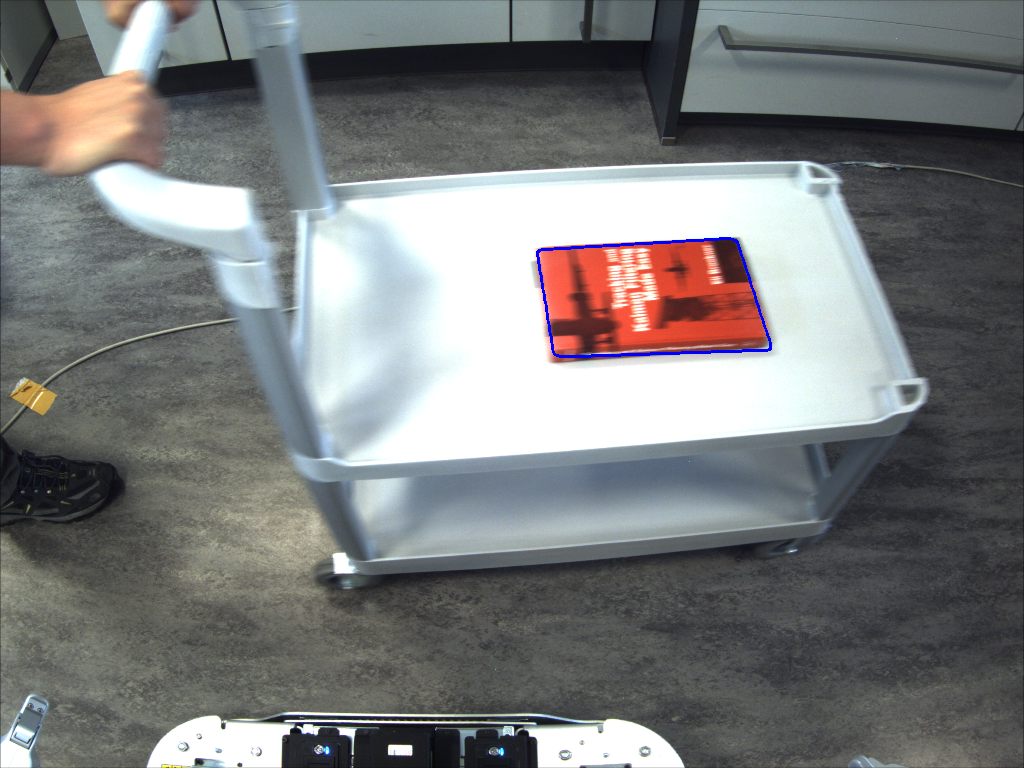
\includegraphics[width=2.5in]{images/sift/45.png}}
  \end{minipage} 
  \begin{minipage}[t]{0.5\linewidth} 
    \centering 
    \subfloat[Sampled frame 5]{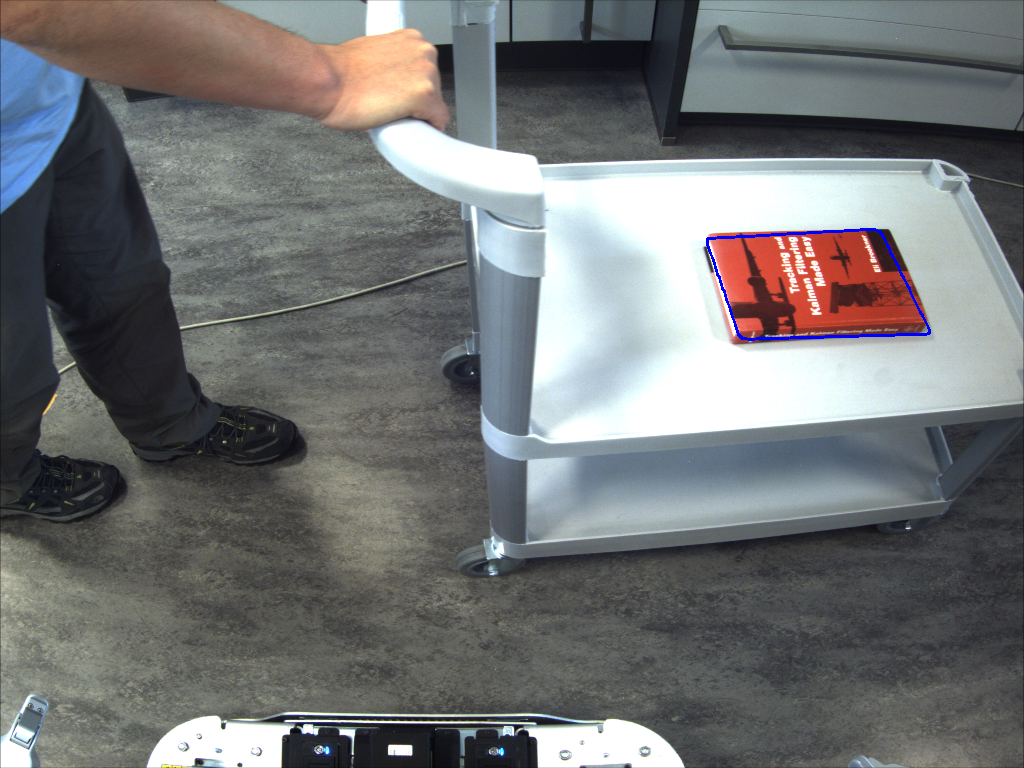
\includegraphics[width=2.5in]{images/sift/63.png}}
  \end{minipage} 
  \begin{minipage}[t]{0.5\linewidth} 
    \centering 
    \subfloat[Sampled frame 6]{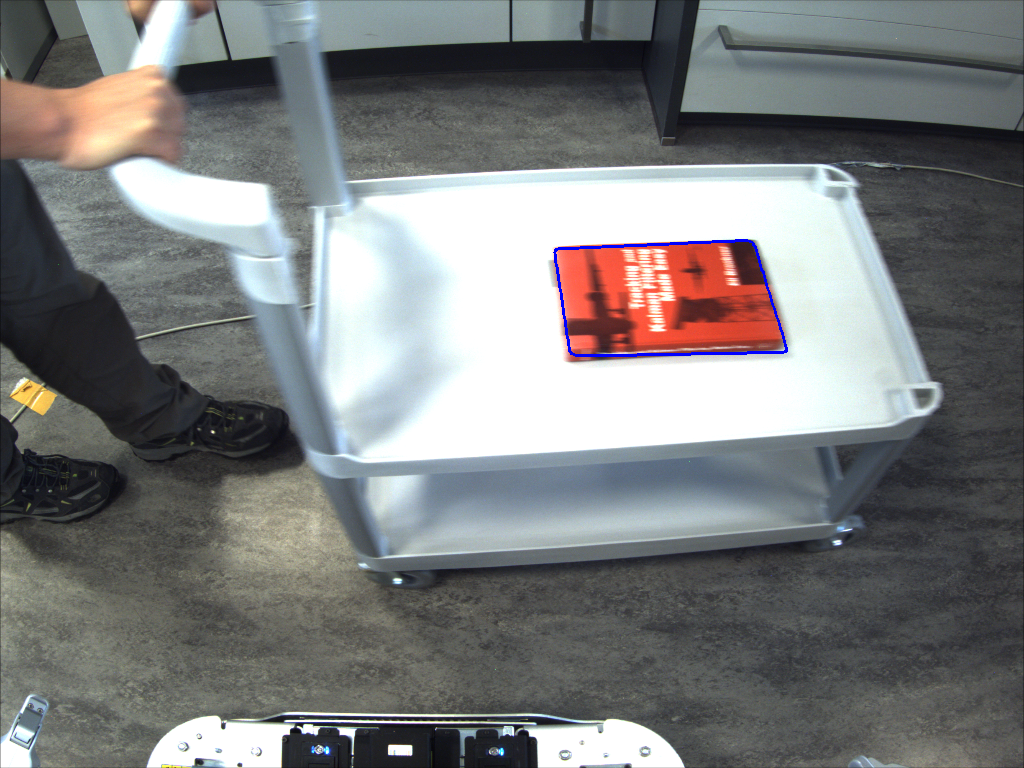
\includegraphics[width=2.5in]{images/sift/80.png}}
  \end{minipage} 
  \caption[The tracking result based on SIFT contour initialization]{The
    CCD tracker successfully tracks the motion of a book. However, in
    sampled frame  5, the contour of the book is not in planar shape-space
    any more, because the given model is a rigid one, the tracker can not
    completely converge to the edge of the book. The better result is
    obtained in sampled frame 6 again.
  }
  \label{fig:sifttracker}
\end{figure}


\section{Track initialization from 3D point cloud}
\label{sec:tifpc}

A point cloud is a set of vertices created by 3-Dimensional
scanners. The scanners measure points on the surface of a object,
therefore, a point cloud represents the set of points measured by the
device. Point clouds cloud are widely used to  create 3D CAD models
for manufactured parts, a multitude of visualization, animation and
rendering.
\begin{figure}[htb]
  \centering
  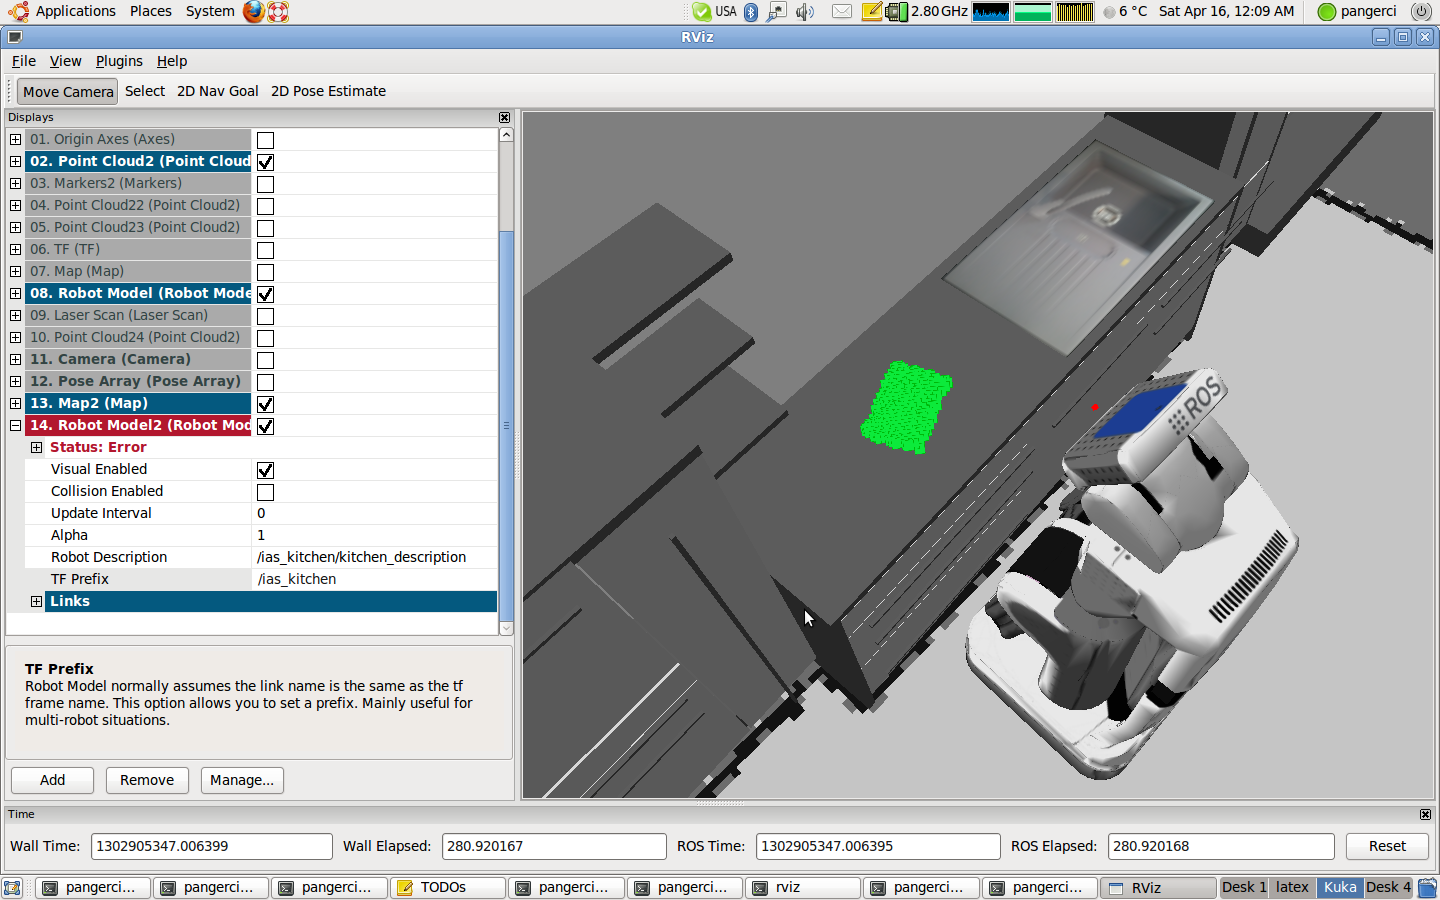
\includegraphics[width=\linewidth]{images/pr2b.png}
  \caption[Point cloud of a book rendered in rivz]{A point cloud is
    generated by the scanner in PR2.}
  \label{fig:pointcloud}
\end{figure}

Point clouds can be rendered and inspected in software like MeshLab
and rivtz (Figure~\ref{fig:pointcloud}). In addition, they are usually converted to polygon or
triangle mesh models, NURBS surface models, or CAD models through a
process commonly referred to as surface reconstruction.

In this experiments, we plan to convert a point cloud of a object to a
polygon, then use this polygon as the initial contour of observed
object. In the point cloud in Figure~\ref{fig:pointcloud}, edges of
the observed object are not smoothed. By applying the CCD algorithm,
we can accurately obtain the contour of a observed object. In
comparison with the initialization from SIFT features, because the
outlines created from point cloud is 3-Dimensional, it is more
suitable for non-planar objects.
